% TEXINPUTS=.:$HOME/git/bvtex: latexmk  -pdf <main>.tex
\documentclass[xcolor=dvipsnames]{beamer}

\input{defaults}

\input{beamer/preamble}
\usepackage[outline]{contour}

\definecolor{bvtitlecolor}{rgb}{0.98, 0.92, 0.84}
\definecolor{bvoutline}{rgb}{0.1, 0.1, 0.1}

\renewcommand{\bvtit}{Wire Cell}
\renewcommand{\bvtitle}{\LARGE Wire Cell Software Overview and Status}
\renewcommand{\bvevent}{BNLIF Wire Cell Team\\ 2015 Aug 11}
\renewcommand{\bvbeamerbackground}{}
\begin{document}
\input{beamer/title.tex}
\input{beamer/toc.tex}


\lstset{%
  language=C++,
                basicstyle=\scriptsize\ttfamily,
                keywordstyle=\color{blue}\ttfamily,
                stringstyle=\color{red}\ttfamily,
                commentstyle=\color{gray}\ttfamily,
                morecomment=[l][\color{magenta}]{\#}
}

\section{Method}

\begin{frame}
  \frametitle{Wire Cell Gestalt}

  \begin{columns}
    \begin{column}{0.6\paperwidth}
      \scriptsize
      \begin{enumerate}
      \item Tile the wire plane with ``cells'', each associated with
        one wire from each plane.
      \item Focus on a time-slice across the readout channels
        (nominally 4 ticks).
      \item Determine which cells may contain charge consistent with
        the sliced readout for their wires.
      \item Merge potential hit cells into ``blobs'' to reduce
        multiplicity.
      \item Attempt to solve a wire-cell association matrix via
        $\chi^2$ minimization.
      \item Associate solution back in time to drift origin to form 3D point.
      \item Clustering, PID, Physics!
      \end{enumerate}
    \end{column}
    \begin{column}{0.4\paperwidth}
      \begin{center}
        \vspace{-1cm}

      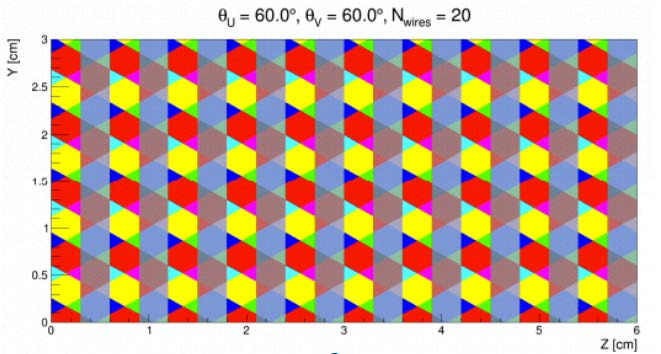
\includegraphics[width=5cm]{cells.png}

      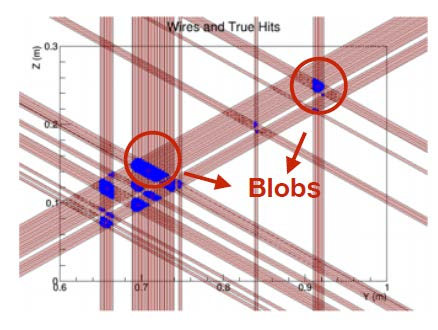
\includegraphics[width=5cm]{blobs.png}
      \end{center}
    \end{column}
  \end{columns}

  \vspace{5mm}
  \footnotesize
  For more information, see:
  \begin{itemize}
  \item \href{https://indico.fnal.gov/getFile.py/access?contribId=3&resId=0&materialId=slides&confId=10240}{Chao
      Zhang's presentation to 35t/FD Sim, Reco, and Analysis}.
    
  \item A detailed paper is in preparation.
  \end{itemize}
\end{frame}

\begin{frame}
  \frametitle{Wire Cell Example Solution, 1.5 GeV $e^-$}
    \begin{columns}
      \begin{column}{0.33\paperwidth}
        \begin{center}
          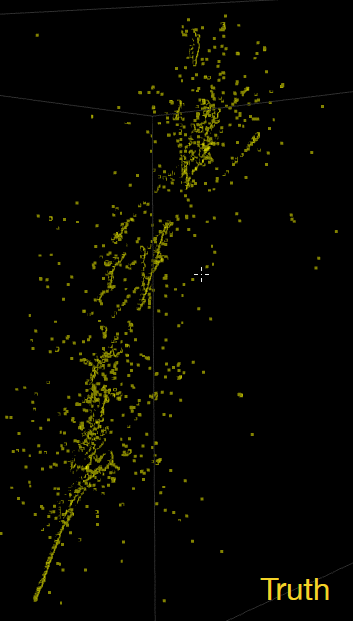
\includegraphics[height=7cm]{ele-truth.png}

          \scriptsize MC depositions.
        \end{center}
      \end{column}
      \begin{column}{0.33\paperwidth}
        \begin{center}
          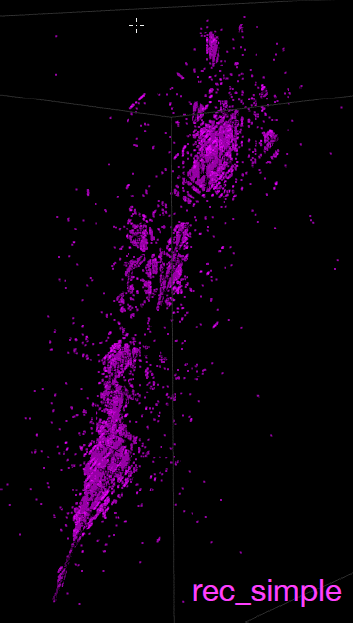
\includegraphics[height=7cm]{ele-simple.png}

          \scriptsize Only geometry
        \end{center}
      \end{column}
      \begin{column}{0.33\paperwidth}
        \begin{center}
          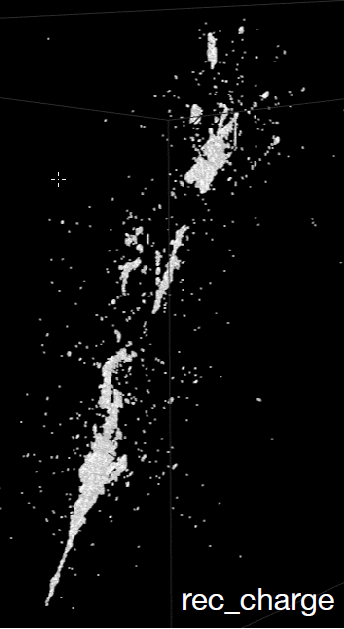
\includegraphics[height=7cm]{ele-charge.png}

          \scriptsize Geometry and charge.
        \end{center}
      \end{column}
    \end{columns}

\end{frame}



\section{Wire Cell Software}

\begin{frame}
  \frametitle{Wire Cell Software Ecosystem}

  Consists roughly of these parts:

  \begin{description}
  \item[bee] 3D interactive web-based event display.
  \item[core] C++ libraries providing:
    \begin{itemize}
    \item data and geometry representations.
    \item the reconstruction procedures themselves.
    \item charge drifting and signal processing.
    \item various data/geometry file I/O.
    \item job configuration and a processing model.
    \end{itemize}
  \item[misc] file-based data exchange with LArSoft,
    stand-alone signal processing studies, experimental clustering,
    bee file server, some others.
  \end{description}

\end{frame}


\begin{frame}[fragile]
  \frametitle{Bee}

  \scriptsize
  \begin{center}
    \vspace{-0.5cm}

    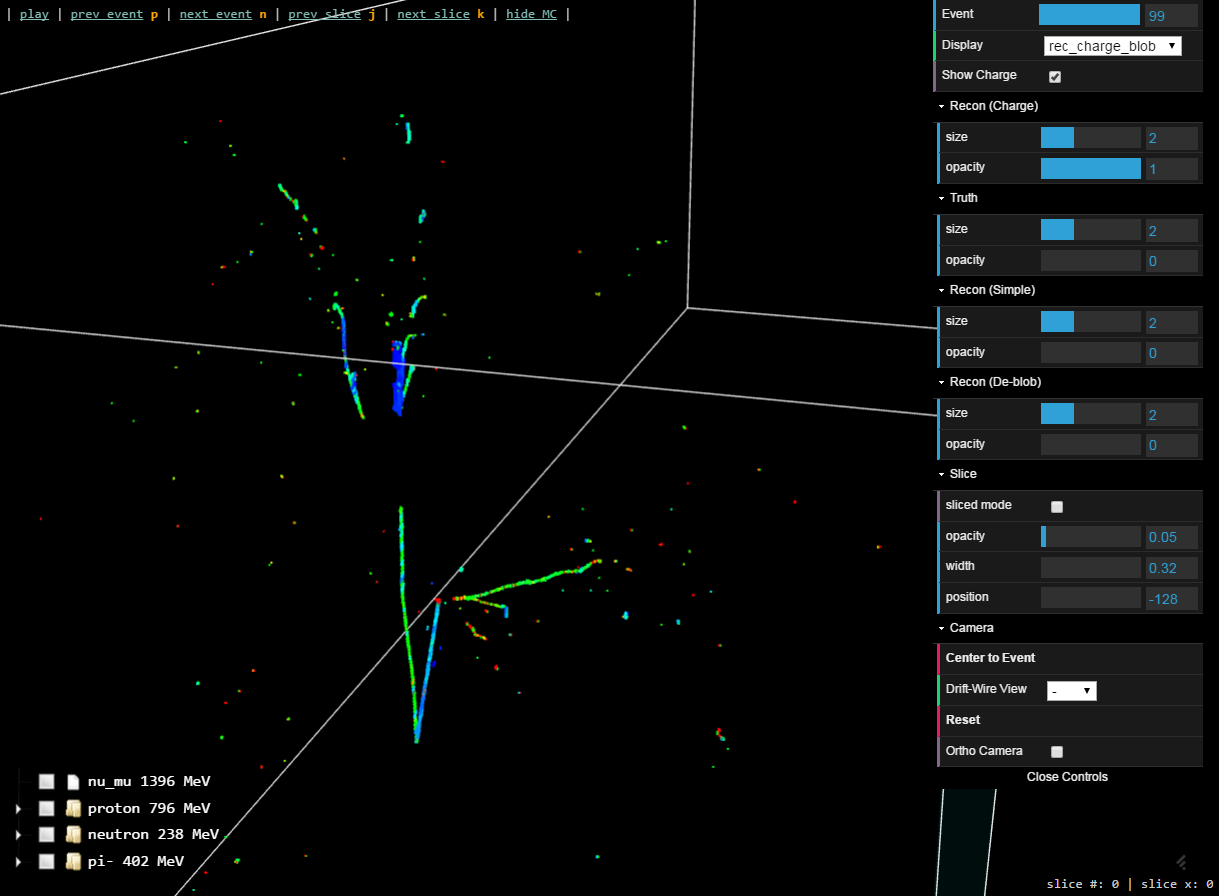
\includegraphics[height=6cm]{bee.png}    

    \url{http://www.phy.bnl.gov/wire-cell/examples/mvd/numu-nc-v2/#/99}
  \end{center}

  \begin{itemize}
  \item 3D, interactive, web-browser interface using WebGL acceleration.
  \item Display MC truth, WC and other reconstruction results,
    simple JSON file format.
  \item Server side file organization and JS delivery based on Django.
  \end{itemize}

\end{frame}

\begin{frame}
  \frametitle{Wire Cell Source Code Repositories} 
  \footnotesize

  The Bee display:
  \begin{itemize}
  \item \href{https://github.com/BNLIF/wire-cell-viz-webgl}{wire-cell-viz-webgl}
    repository.
  \item Primary developer: Chao.
  \end{itemize}

  \vspace{5mm}

  Wire Cell ``core'' repositories have \textbf{two active branches}:
  \begin{description}
  \item[master] \textbf{working prototype} code producing the results we've
    been showing, (primary: Xin).
  \item[ifaceio] fork of \texttt{master}, for \textbf{structured,
      production code} for long term development, tuning and toward
    supporting parallel architectures, (primary: bv).
  \end{description}

  \vspace{10mm}
  \scriptsize
  \flushright Focus on Wire Cell ``core'' parts next $\rightarrow$
\end{frame}


\begin{frame}
  \frametitle{Installation of Wire Cell ``core''}

  Primary dependencies (subject to change):
  \begin{description}
  \item[build:] C++11 compiler (GCC 4.9.2 used)
  \item[core:] Boost (1.55)
  \item[apps/tests:] ROOT 6 (6.05/01)
  \end{description}

  \vspace{5mm}

  Some build details:
  \begin{itemize}
  \item Source packages aggregated via \texttt{git submodules}
  \item Native build system: \href{https://waf.io/}{waf}
    (self-contained copy provided).
  \item Unit and integration tests run regularly as part of the build.
  \item Installs shared libraries + headers + few main applications.
  \end{itemize}
  
  \vspace{5mm}
  \scriptsize
  Details at \url{http://bnlif.github.io/wire-cell-docs/install/}.
\end{frame}



\begin{frame}
  \frametitle{Wire Cell ``core'' Packages Overview}

  \footnotesize

  Wire Cell core packages, most named like \texttt{wire-cell-*}:

  \begin{description}
  \item[wire-cell] \texttt{git submodule} aggregation and top-level build-package,
    (\href{https://github.com/BNLIF/wire-cell/}{\texttt{master}},
    \href{https://github.com/BNLIF/wire-cell/tree/ifaceio/}{\texttt{ifaceio}}).
  \item[-data] common, concrete data
    classes, (\href{https://github.com/BNLIF/wire-cell-data/}{\texttt{master}}).
  \item[-2dtoy] working prototype implementation,
    (\href{https://github.com/BNLIF/wire-cell-2dtoy}{\texttt{master}}).
  \item[-util] general utility code, 3D vector, system of units,
    configuration files, various C++ patterns,
    (\href{https://github.com/BNLIF/wire-cell-util/tree/ifaceio}{\texttt{ifaceio}}).
  \item[-iface] interface classes for major components and data
    classes, 
    (\href{https://github.com/BNLIF/wire-cell-iface/tree/ifaceio}{\texttt{ifaceio}}).
  \item[-nav] default implementation of wire cell components with
    minimal outside dependencies, (\href{https://github.com/BNLIF/wire-cell-nav/}{\texttt{master}},
    \href{https://github.com/BNLIF/wire-cell-nav/tree/ifaceio/}{\texttt{ifaceio}}).
  \item[-rio] internal ROOT I/O persistency,
    (\href{https://github.com/BNLIF/wire-cell-rio/tree/ifaceio/}{\texttt{ifaceio}}).
  \item[-sst] ``simple simulation tree'' file-interface to use LArSoft
    data and geometry as one possible input to Wire Cell,
    (\href{https://github.com/BNLIF/wire-cell-sst/}{\texttt{master}},
    \href{https://github.com/BNLIF/wire-cell-sst/tree/ifaceio/}{\texttt{ifaceio}}).
  \item[waf-tools] \texttt{waf} support files for the native build
    system,
    (\href{https://github.com/BNLIF/waf-tools/}{\texttt{master}},
    \href{https://github.com/BNLIF/waf-tools/tree/ifaceio/}{\texttt{ifaceio}}).

  \end{description}
  All found at \url{https://github.com/BNLIF/}.
  
\end{frame}

\begin{frame}[fragile]
  \frametitle{Wire Cell Class Interfaces}

  \vspace{5mm}
  \footnotesize

  \begin{itemize}
  \item All important Wire Cell classes (in \texttt{ifaceio}) inherit
    from abstract base classes following \textbf{Interface} patterns.
  \item Interface methods take POD or Interfaces.
  \item Code is in the \texttt{wire-cell-iface} package.
  \item \verb|std::shared_ptr<>| memory ownership rules,
  \end{itemize}

  \footnotesize

  Two main categories of interfaces:
  \begin{description}
  \item[data] (eg, \texttt{ICell}, \texttt{ISlice})
    \begin{itemize}
    \item Data is const once created.
    \item Abstract iterator interface for collections.
    \end{itemize}
  \item[component] (eg, \texttt{IConfigurable}, \texttt{IWireSummary},
    \texttt{ITiling})
    \begin{itemize}
    \item Interface defines a facet of functionality.
    \item Name-based location/construction to support job
      configuration and loosely coupled build dependencies.
    \end{itemize}
  \end{description}


\end{frame}

\begin{frame}
  \frametitle{Data Flow Programming Paradigm}

  \begin{columns}
    \footnotesize
    \begin{column}{0.5\paperwidth}
      Wire Cell supports the ``data flow programming'' paradigm.
      \scriptsize
      \begin{itemize}
      \item Components are written to provide well formed ``sockets''
        (methods) connected to accepting ``signals''.
      \item Connections prototypes are standardized based on purpose.
      \item Execution model is synchronous ``pull''.
      \item Potential  for
        fine-grained parallel execution model with no component code changes. 
      \item Now, connections formed in C++ but this will be exported
        to the end-user configuration layer.        
      \end{itemize}
    \end{column}
    \begin{column}{0.4\paperwidth}
      \begin{center}
        \vspace{-1cm}

        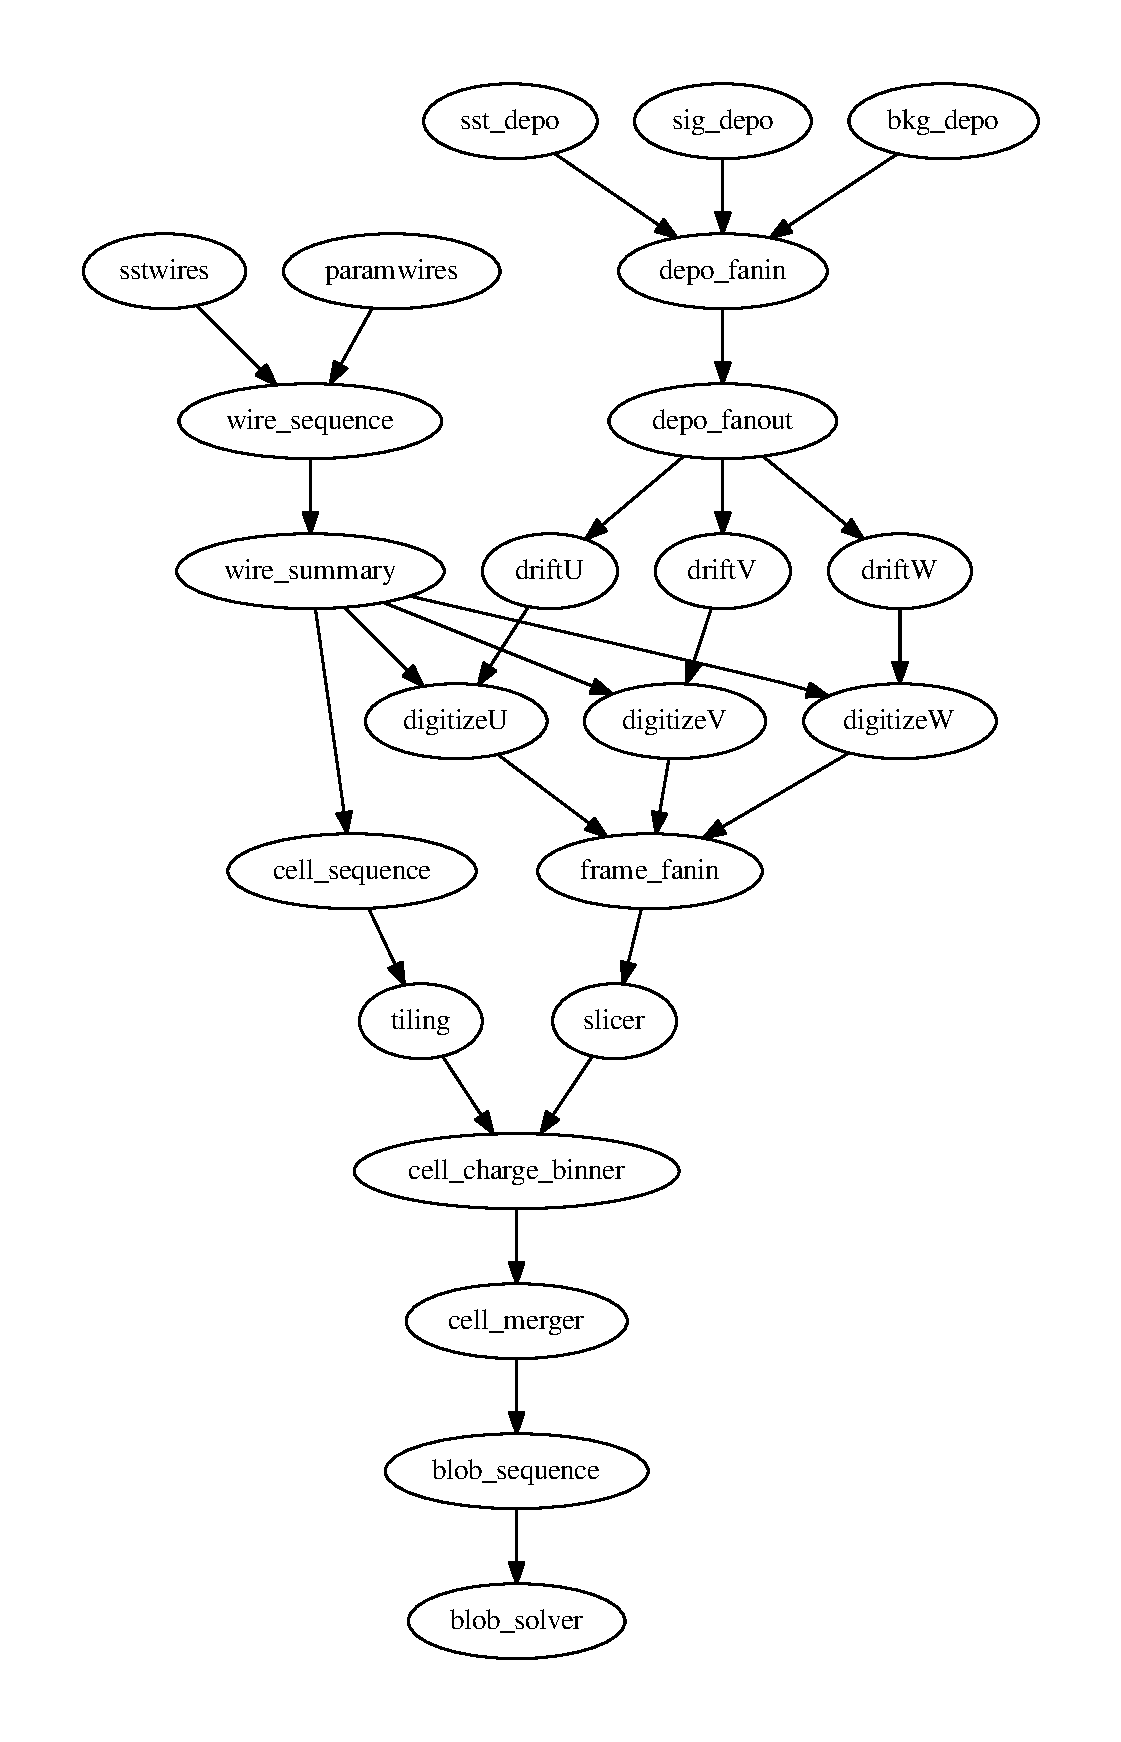
\includegraphics[height=8cm]{dataflow.pdf}
      \end{center}
      
    \end{column}
  \end{columns}
\end{frame}

\section{Connections with LArSoft}

\begin{frame}
  \frametitle{Current Wire Cell / LArSoft Integration}

  \begin{columns}
    \begin{column}{0.7\paperwidth}
      \scriptsize
      \begin{itemize}
      \item Wire Cell (core) is wholly independent from LArSoft.
      \item Stand-alone deposition, drifting, digitizing, etc provided.
      \item Deposition/digit/geometry input from other simulations possible.
      \end{itemize}

      \vspace{2mm}

      Existing LArSoft integration is via exchange files:
      \begin{itemize}
      \item The \texttt{celltree} LArSoft module, (Chao).
      \item Produces a plain ROOT TTree with (hits, digits) and dumps
        wire geometry (as text).
      \item Independent from Wire Cell software.
      \item Not committed, needs a LArSoft package to call home (\textbf{suggestions?}).
      \item Module is not specific to one LArSoft-supported detector.
      \item Files read in by \texttt{wire-cell-sst} package.
      \item A module to read back Wire Cell output file into to LArSoft is in development.
        \begin{itemize}
          \scriptsize
        \item[$\rightarrow$] Need \textbf{new charge+point data product}
          in LArSoft!
        In mean time, will try to populate closest suitable data products.
        \end{itemize}
      \end{itemize}
      
    \end{column}
    \begin{column}{0.2\paperwidth}
      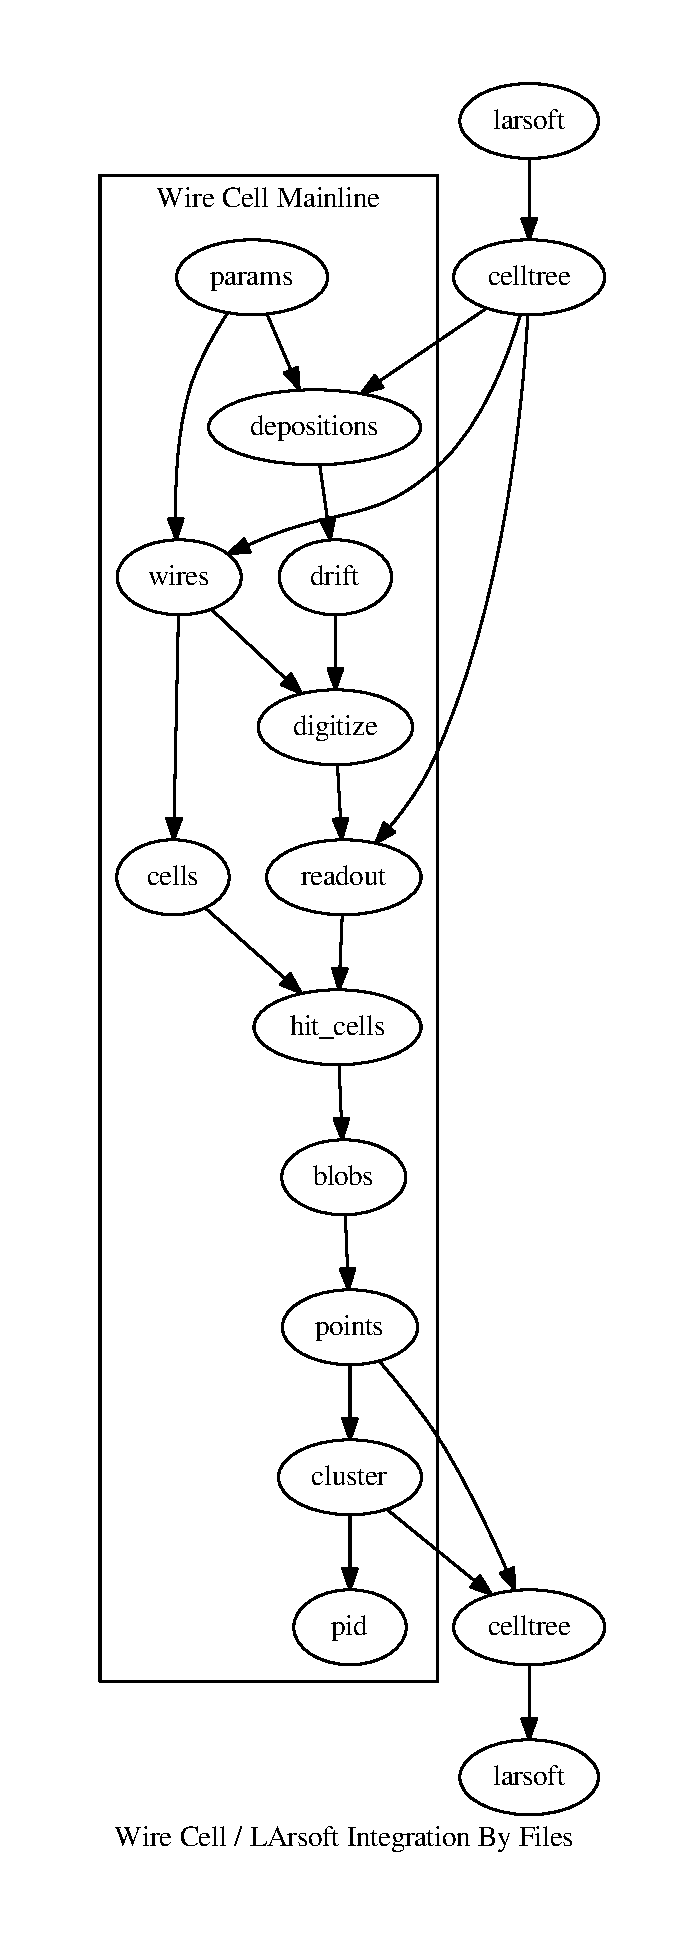
\includegraphics[height=8cm]{wc-ls.pdf}
    \end{column}
  \end{columns}
\end{frame}

\begin{frame}
  \frametitle{Future Wire Cell / LArSoft Integration}

  \scriptsize

  \textbf{Main technical challenges}:
  \begin{itemize}
  \item Both Wire Cell and LArSoft require a large amount
    of \textbf{memory}.
  \item We expect Wire Cell to be a significant \textbf{CPU} bottleneck
  \end{itemize}

  Our strategy is to make Wire Cell run in \textbf{fine-grained parallel}.
  \begin{itemize}
  \item Parallel at the \textbf{time slice} or even the lower ``\textbf{blob}'' level.
  \item Possible \textbf{GPU} acceleration, possible \textbf{HPC} utilization.
  \item Further integration with LArSoft must be understood is in this context.
  \end{itemize}

  Options:
  \begin{itemize}
  \item Maybe employ \textbf{ATLAS Event Service} approach (actual or DIY)?
    \begin{itemize}
    \scriptsize
    \item Need to understand how LArSoft ``mothership'' communicates to many
      instances of Wire Cell.
    \end{itemize}
  \item Enact parallel compute units in the \textbf{data flow programming} paradigm?
    \begin{itemize}
    \scriptsize
    \item Need parallel execution framework (exists but needs testing)
    \end{itemize}
  \end{itemize}

  In any case, let's start by \textbf{developing a ``\texttt{LarWireCell}'' module}:
  \begin{itemize}
  \item Wire Cell (core) remains LArSoft ``\textbf{external}'' and needs UPS packaging.
    \begin{itemize}
      \tiny
    \item Mimic Pandora's integration patterns.
    \end{itemize}
  \item A LArSoft module needs to convert between data representations
    and all Wire Cell methods.
  \item I hope a \textbf{LArSoft expert} is interested in helping with this!
  \end{itemize}


\end{frame}

\section{}

\begin{frame}
  \frametitle{Summary}
  \begin{itemize}
  \item A working prototype clearly shows the power of the Wire Cell technique.
  \item A code-refactoring is in progress to provide needed structure going forward.
  \item Initial samples of 1000s of events have been processed and are
    available via the Bee online event display.
  \end{itemize}
  Future directions:
  \begin{itemize}
  \item \textbf{Expert help needed} to improve integration with
    LArSoft!
  \item Capture existing \textbf{file-based integration methods} into some
    LArSoft package.
  \item Explore how to tackle \textbf{significant technical
      challenges} driven by the expected high CPU requirements and in
    the face of memory pressures from both LArSoft and Wire Cell.
  \end{itemize}
\end{frame}

\begin{frame}
  \frametitle{Online Entry Points for More Info}
  The Wire Cell home page collects all info:
  \begin{center}
    \url{http://www.phy.bnl.gov/wire-cell/}    
  \end{center}
  Including links to:
  \begin{itemize}
  \item \href{http://www.phy.bnl.gov/wire-cell/examples/list/}{Bee online
      3d event display}
  \item \href{http://bnlif.github.io/wire-cell-docs/}{Software documentation}
  \item \href{https://github.com/BNLIF/wire-cell/}{Software repositories}
  \end{itemize}
\end{frame}

\end{document}

